% !TEX program = pdflatex
\documentclass[aspectratio=169,10pt]{beamer}
\usetheme[progressbar=frametitle,numbering=fraction,background=light]{metropolis}
\usepackage[T1]{fontenc}

\usepackage{amsmath,amssymb,booktabs,array,listings,xcolor,graphicx}
\usepackage{tikz,pgfplots}
\pgfplotsset{compat=1.17}
\usetikzlibrary{arrows.meta,positioning,shapes.geometric,fit,calc,backgrounds,decorations.pathmorphing}

\definecolor{navy}{HTML}{1F3A5F}\definecolor{teal}{HTML}{1B8A8F}
\definecolor{amber}{HTML}{D98E04}\definecolor{crimson}{HTML}{B3263E}
\definecolor{violet}{HTML}{6A4C9C}\definecolor{green}{HTML}{3A8F4B}
\setbeamercolor{progress bar}{fg=teal,bg=teal!20}
\setbeamercolor{frametitle}{bg=navy}
\setbeamercolor{block title}{bg=navy!85,fg=white}
\setbeamercolor{block body}{bg=navy!6}
\setbeamercolor{block title alerted}{bg=crimson!85,fg=white}
\setbeamercolor{block body alerted}{bg=crimson!6}
\setbeamercolor{block title example}{bg=teal!85,fg=white}
\setbeamercolor{block body example}{bg=teal!7}
\setbeamerfont{block title}{size=\small}
\setbeamerfont{block body}{size=\small}

\renewcommand{\Pr}{\mathbb{P}}
\newcommand{\E}{\mathbb{E}}
\newcommand{\sone}{\textsc{S1}}\newcommand{\stwo}{\textsc{S2}}
\newtheorem{proposition}{Proposition}
\newcommand{\thm}[1]{\textcolor{crimson}{\textbf{#1}}}

\tikzset{
 blk/.style={rounded corners=3pt,draw=#1!80!black,fill=#1!12,thick,align=center,font=\scriptsize,minimum width=2.3cm,minimum height=0.8cm,inner sep=3pt},
 arr/.style={-{Stealth[length=4pt]},thick,draw=black!70},
 dsh/.style={-{Stealth[length=4pt]},thick,dashed,draw=black!55},
 lab/.style={font=\tiny,fill=white,inner sep=1pt,text=black!75}
}
\pgfplotsset{every axis/.append style={font=\scriptsize,grid=major,grid style={black!10},width=\linewidth,height=4.5cm,legend style={font=\tiny,draw=none,fill=white,fill opacity=.8,text opacity=1}}}
\lstset{basicstyle=\ttfamily\scriptsize,backgroundcolor=\color{navy!5},frame=single,rulecolor=\color{navy!30},keywordstyle=\color{crimson}\bfseries,commentstyle=\color{teal},showstringspaces=false,morekeywords={def,return,if,and,or,not}}

\title{Nafs-Aql v0.1}
\subtitle{Mathematical validation and technical report of a dual-process agent on Qwen\\[2pt]\footnotesize System 1 (fast) $\cdot$ System 2 (slow) $\cdot$ Active-Intellect verifiers $\cdot$ value core $\cdot$ gated distillation}
\author{Architecture review of the Technical Specification, Model Choices note and Validation Addendum}
\date{18 October 2026}

\begin{document}
\maketitle

\begin{frame}{Outline}
\begin{columns}[T]
\column{.5\textwidth}
\textbf{Part I -- Problem and architecture}
\begin{itemize}\small
\item Executive verdict
\item Concept map and data flow
\item Qwen roster and serving
\item Formal setting and assumptions
\end{itemize}
\textbf{Part II -- Validation (12 results)}
\begin{itemize}\small
\item Verifier, best-of-$N$, cascade cost
\item Router, consensus, value core
\item Coupling, self-model, measurement floors
\item Distillation, serving, end-to-end identity
\end{itemize}
\column{.5\textwidth}
\textbf{Part III -- Technical report}
\begin{itemize}\small
\item Defect register and amended design
\item Features and capabilities
\item Revised constants and gates
\item Development plan, risks, open items
\end{itemize}
\vspace{4pt}
\begin{alertblock}{Method}
Every numeric claim of the addendum was recomputed independently (all reproduced). Extra results added here: heterogeneity gap for T2 and the cascade difference identity (P1).
\end{alertblock}
\end{columns}
\end{frame}

\section{Part I: Problem and architecture}

\begin{frame}{Executive verdict}
\begin{columns}[T]
\column{.48\textwidth}
\begin{block}{Verdict}
\textbf{Buildable on Qwen: yes, with amendments.}\\
The structure is sound: cheap policy $\to$ calibrated router $\to$ verified best-of-$N$ $\to$ scoring judge $\to$ metrics-only self-model $\to$ gated distillation.
\end{block}
\begin{exampleblock}{What holds}
\small
\begin{itemize}
\item Roster is implementable (embedding/reranker versions and MoE-LoRA are the open risks)
\item Verifier-grounded loop is the right core
\item Metrics-only self-model blocks confabulation
\item Human-signed promotion limits drift
\end{itemize}
\end{exampleblock}
\column{.52\textwidth}
\begin{alertblock}{Ten defects found in text, code and thresholds}
\scriptsize
\begin{enumerate}
\item Cascade beats S2-only only if escalation $\lesssim 5\%$ (T3); baseline undefined
\item 500-task baseline too small for most gates
\item Hard gate not coded; vacuous hedge scores 0.75
\item $V_{\min}{=}0.9$ lets code fail 10\% of tests; consensus $\Rightarrow$ unanimity
\item $\tau$ adapted to target $g$, yet $g$ is the learning diagnostic
\item Self-model biased by routing selection
\item ECE gate 0.08 unmeasurable at $n{=}500$
\item S1 draft passed to S2 invites anchoring
\item Math verifier lists LLM rederivation
\item Router pseudo-code $\neq$ prose rule
\end{enumerate}
\end{alertblock}
\end{columns}
\end{frame}

\begin{frame}{Concept map: from philosophy to modules}
\centering
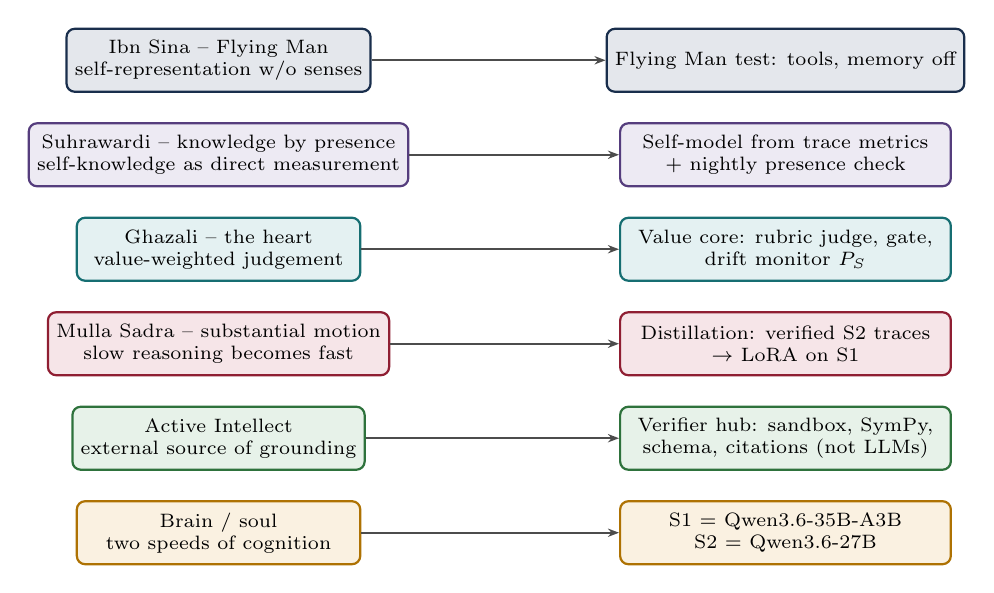
\begin{tikzpicture}[x=1cm,y=1cm]
\node[blk=navy,minimum width=3.6cm] (a) at (0,3.4) {Ibn Sina -- Flying Man\\ self-representation w/o senses};
\node[blk=violet,minimum width=3.6cm] (b) at (0,2.2) {Suhrawardi -- knowledge by presence\\ self-knowledge as direct measurement};
\node[blk=teal,minimum width=3.6cm] (c) at (0,1.0) {Ghazali -- the heart\\ value-weighted judgement};
\node[blk=crimson,minimum width=3.6cm] (d) at (0,-0.2) {Mulla Sadra -- substantial motion\\ slow reasoning becomes fast};
\node[blk=green,minimum width=3.6cm] (e) at (0,-1.4) {Active Intellect\\ external source of grounding};
\node[blk=amber,minimum width=3.6cm] (f) at (0,-2.6) {Brain / soul\\ two speeds of cognition};
\node[blk=navy,minimum width=4.2cm] (a2) at (7.2,3.4) {Flying Man test: tools, memory off};
\node[blk=violet,minimum width=4.2cm] (b2) at (7.2,2.2) {Self-model from trace metrics\\ + nightly presence check};
\node[blk=teal,minimum width=4.2cm] (c2) at (7.2,1.0) {Value core: rubric judge, gate,\\ drift monitor $P_S$};
\node[blk=crimson,minimum width=4.2cm] (d2) at (7.2,-0.2) {Distillation: verified S2 traces\\ $\to$ LoRA on S1};
\node[blk=green,minimum width=4.2cm] (e2) at (7.2,-1.4) {Verifier hub: sandbox, SymPy,\\ schema, citations (not LLMs)};
\node[blk=amber,minimum width=4.2cm] (f2) at (7.2,-2.6) {S1 = Qwen3.6-35B-A3B\\ S2 = Qwen3.6-27B};
\foreach \i in {a,b,c,d,e,f}{\draw[arr] (\i.east) -- (\i2.west);}
\end{tikzpicture}

\vspace{2pt}\scriptsize Metaphor only: the project makes no claim of consciousness. The formal content is in Part II.
\end{frame}

\begin{frame}{System architecture and data flow}
\centering
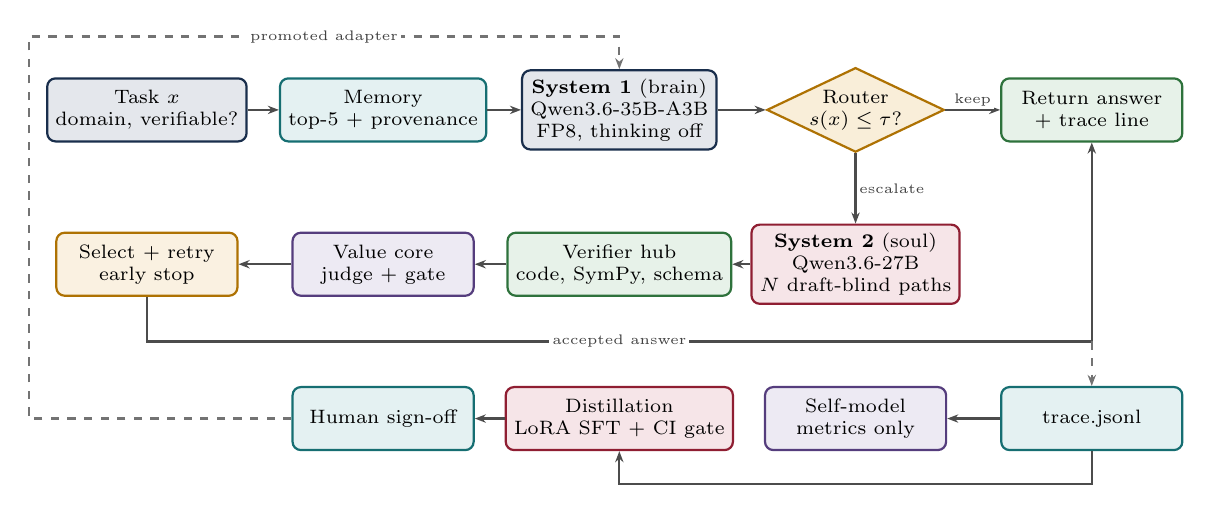
\begin{tikzpicture}[x=1.0cm,y=0.98cm]
\node[blk=navy] (task) at (0,0) {Task $x$\\ domain, verifiable?};
\node[blk=teal] (mem) at (3,0) {Memory\\ top-5 + provenance};
\node[blk=navy] (s1) at (6,0) {\textbf{System 1} (brain)\\ Qwen3.6-35B-A3B\\ FP8, thinking off};
\node[diamond,aspect=2.1,draw=amber!80!black,fill=amber!15,thick,font=\scriptsize,align=center,inner sep=0pt] (rt) at (9,0) {Router\\ $s(x)\le\tau$?};
\node[blk=green] (out) at (12,0) {Return answer\\ + trace line};
\node[blk=crimson] (s2) at (9,-2) {\textbf{System 2} (soul)\\ Qwen3.6-27B\\ $N$ draft-blind paths};
\node[blk=green] (ver) at (6,-2) {Verifier hub\\ code, SymPy, schema};
\node[blk=violet] (val) at (3,-2) {Value core\\ judge + gate};
\node[blk=amber] (sel) at (0,-2) {Select + retry\\ early stop};
\node[blk=teal] (log) at (12,-4) {trace.jsonl};
\node[blk=violet] (sm) at (9,-4) {Self-model\\ metrics only};
\node[blk=crimson] (dist) at (6,-4) {Distillation\\ LoRA SFT + CI gate};
\node[blk=teal] (hum) at (3,-4) {Human sign-off};
\draw[arr] (task)--(mem);\draw[arr] (mem)--(s1);\draw[arr] (s1)--(rt);
\draw[arr] (rt)--node[lab,above]{keep}(out);
\draw[arr] (rt)--node[lab,right]{escalate}(s2);
\draw[arr] (s2)--(ver);\draw[arr] (ver)--(val);\draw[arr] (val)--(sel);
\draw[arr] (sel.south)--(0,-3)--node[lab]{accepted answer}(12,-3)--(out.south);
\draw[dsh] (12,-3)--(log.north);
\draw[arr] (log)--(sm);
\draw[arr] (log.south)--(12,-4.85)--(6,-4.85)--(dist.south);
\draw[arr] (dist)--(hum);
\draw[dsh] (hum.west)--(-1.5,-4)--(-1.5,0.95)--node[lab]{promoted adapter}(6,0.95)--(s1.north);
\end{tikzpicture}
\end{frame}

\begin{frame}{Qwen roster and serving profile}
\begin{columns}[T]
\column{.54\textwidth}
\scriptsize
\begin{tabular}{@{}p{1.5cm}p{2.3cm}p{2.7cm}@{}}
\toprule
Role & Model & Mode / status\\\midrule
System 1 & Qwen3.6-35B-A3B (MoE, ${\sim}3$B active) & thinking off; official FP8 repo; card details to confirm\\
System 2 & Qwen3.6-27B dense, Apache 2.0, 262K ctx & thinking on, \texttt{preserve\_thinking}\\
Value core & same 27B weights & thinking off, rubric, $T{=}0$\\
Embed / rerank & Qwen3-Embedding-4B, Reranker-4B & \textbf{unverified}; read dim from config\\
Verifiers & sandbox, SymPy, JSON-Schema & deterministic, non-LLM\\\bottomrule
\end{tabular}

\vspace{4pt}
\begin{alertblock}{Pin and re-baseline}
Pin exact revisions. Any change of model, template or adapter re-runs the Phase~0 baseline. Do not chase Qwen3.7/3.8/4 mid-build.
\end{alertblock}
\column{.46\textwidth}
\centering\scriptsize Profile A memory budget (80\,GB GPUs, util 0.90)\\[2pt]
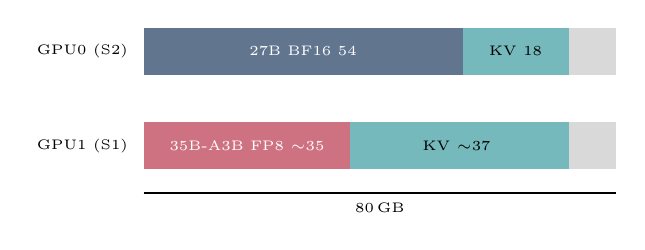
\begin{tikzpicture}[x=0.075cm,y=1cm]
\node[anchor=east,font=\tiny] at (-1,0.6){GPU0 (S2)};
\fill[navy!70](0,0.3) rectangle (54,0.9);\node[white,font=\tiny] at (27,0.6){27B BF16 54};
\fill[teal!60](54,0.3) rectangle (72,0.9);\node[font=\tiny] at (63,0.6){KV 18};
\fill[black!15](72,0.3) rectangle (80,0.9);
\node[anchor=east,font=\tiny] at (-1,-0.6){GPU1 (S1)};
\fill[crimson!65](0,-0.9) rectangle (35,-0.3);\node[white,font=\tiny] at (17.5,-0.6){35B-A3B FP8 ${\sim}35$};
\fill[teal!60](35,-0.9) rectangle (72,-0.3);\node[font=\tiny] at (53,-0.6){KV ${\sim}37$};
\fill[black!15](72,-0.9) rectangle (80,-0.3);
\draw[thick](0,-1.2)--(80,-1.2);\node[font=\tiny,below] at (40,-1.2){80\,GB};
\end{tikzpicture}

\vspace{4pt}\scriptsize
Profile B (48\,GB, 4-bit) is development-only: no benchmarking.\\[3pt]
\begin{exampleblock}{Per-request switches}
\scriptsize S1: \texttt{enable\_thinking=False}\\
S2: \texttt{enable\_thinking=True, preserve\_thinking=True}\\
S1 served without a reasoning parser.
\end{exampleblock}
\end{columns}
\end{frame}

\begin{frame}{Formal setting}
\begin{columns}[T]
\column{.55\textwidth}
\begin{definition}[Objects]\small
Task $x$; $C_1,C_2$ = events that the S1 draft / S2 answer is correct.
A verifier accepts a correct answer w.p.\ $r$ (true-accept) and a wrong one w.p.\ $\varphi$ (false-accept).
$q(x)$ = P(one S2 path correct); $N$ paths, $R$ retries, $k$ agreement samples; $c_1,c_p$ = cost of one S1 call / S2 path; $g$ = escalation rate; $s(x)$ = router score.
\end{definition}
\begin{block}{Goal}\small
Maximise verified accuracy subject to expected cost, i.e.
$\min\; \Pr[\text{final wrong}] + \lambda\,\E[\text{cost}]$ over router $\pi$, selector $\sigma$, and S1 weights $\theta$ (via distillation).
\end{block}
\column{.45\textwidth}
\begin{alertblock}{Assumptions}
\small
\begin{description}\setlength{\itemsep}{1pt}
\item[A1] S2 paths conditionally i.i.d.\ given $x$
\item[A2] $(r,\varphi)$ identical for every candidate source
\item[A3] verifiers see only task + final answer
\item[A4] held-out data $\sim$ deployment
\end{description}
\end{alertblock}
\small
\textbf{Weak points:} A1 and A2 (shared weights, Goodhart pressure). Each result states what breaks if they fail.
\end{columns}
\end{frame}

\section{Part II: Validation}

\begin{frame}{T1 -- Precision of a verified return}
\begin{columns}[T]
\column{.5\textwidth}
\begin{theorem}[T1]\small
Prior correctness $p$. Then
$\displaystyle\rho=\Pr[\text{wrong}\mid\text{accepted}]=\frac{\varphi(1-p)}{\varphi(1-p)+rp}$.
$\rho\le\varepsilon \iff \varphi\le\dfrac{\varepsilon\,r\,p}{(1-\varepsilon)(1-p)}$.
\end{theorem}
\small\textit{Proof.} Bayes' rule. \hfill$\square$

\vspace{3pt}
\textbf{Consequence.} Hard tasks $p{=}0.10$, $r{=}0.98$, $\varepsilon{=}0.01$ need $\varphi\le0.0011$; with $\varphi{=}0.02$, $\rho=0.155$.

\begin{alertblock}{Design verdict}
Grounding is limited by verifier $\varphi$, not by model strength. Every verifier must publish $(r,\varphi)$ from \emph{mutation testing}.
\end{alertblock}
\column{.5\textwidth}
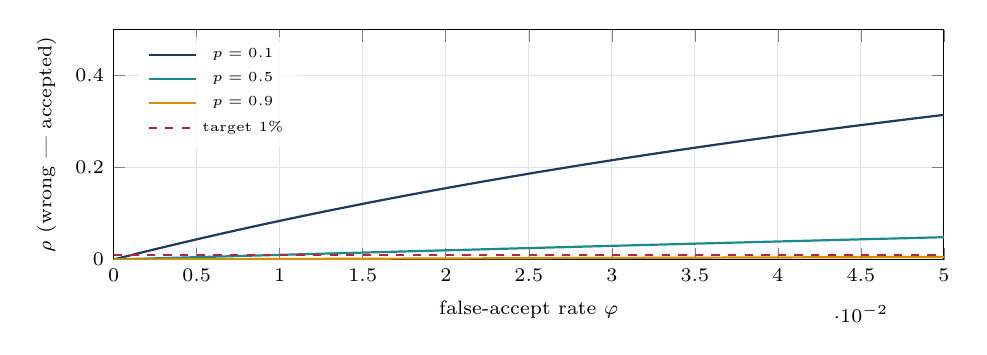
\begin{tikzpicture}
\begin{axis}[xlabel={false-accept rate $\varphi$},ylabel={$\rho$ (wrong | accepted)},xmin=0,xmax=0.05,ymin=0,ymax=0.5,legend pos=north west]
\addplot[navy,thick,domain=0:0.05,samples=60]{x*0.9/(x*0.9+0.098)};\addlegendentry{$p=0.1$}
\addplot[teal,thick,domain=0:0.05,samples=60]{x*0.5/(x*0.5+0.49)};\addlegendentry{$p=0.5$}
\addplot[amber,thick,domain=0:0.05,samples=60]{x*0.1/(x*0.1+0.882)};\addlegendentry{$p=0.9$}
\addplot[crimson,dashed,thick]coordinates{(0,0.01)(0.05,0.01)};\addlegendentry{target 1\%}
\end{axis}
\end{tikzpicture}
\end{columns}
\end{frame}

\begin{frame}{T2 -- Best-of-$N$ buys coverage, not precision}
\begin{columns}[T]
\column{.5\textwidth}
\begin{theorem}[T2]\small
$a=qr+(1-q)\varphi$. Uniform pick among accepted paths:\\
(i) $\Pr[\text{wrong}\mid\ge1\text{ accepted}]=(1-q)\varphi/a$ for every $N$;\\
(ii) coverage with $M=N(R{+}1)$ draws is $1-(1-a)^M$;\\
(iii) if $q$ varies, coverage $\le 1-(1-\E[a])^M$.
\end{theorem}
\small\textit{Proof.} (i) accepted paths are i.i.d.\ wrong w.p.\ $(1-q)\varphi/a$; (ii) geometric; (iii) $u\mapsto(1-u)^M$ convex, Jensen. $\square$

\textbf{Example} ($q{=}.1$): error stays $15.5\%$; coverage $62.7\%$ at $M{=}8$, $94.8\%$ at $M{=}24$ if homogeneous.\\
\textbf{Added check:} half the tasks $q{=}0$, half $q{=}0.2$ (same $\E[a]$) gives only $69\%$ at $M{=}24$.
\column{.5\textwidth}
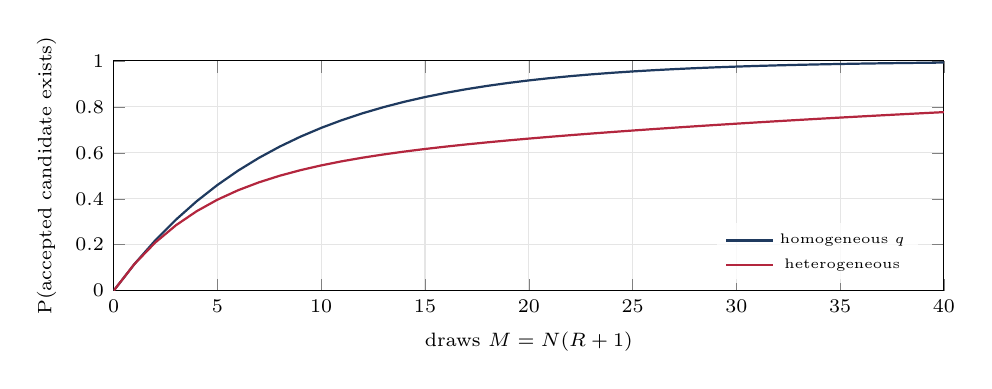
\begin{tikzpicture}
\begin{axis}[xlabel={draws $M=N(R+1)$},ylabel={P(accepted candidate exists)},xmin=0,xmax=40,ymin=0,ymax=1,legend pos=south east]
\addplot[navy,thick,domain=0:40,samples=41]{1-(0.884)^x};\addlegendentry{homogeneous $q$}
\addplot[crimson,thick,domain=0:40,samples=41]{1-0.5*(0.788)^x-0.5*(0.98)^x};\addlegendentry{heterogeneous}
\end{axis}
\end{tikzpicture}

\scriptsize\textbf{Amendment:} choose $N$ from the coverage target; select by score only if it carries information beyond the pass bit; stop at first accepted path on verifiable tasks.
\end{columns}
\end{frame}

\begin{frame}{T3 -- Cascade cost and break-even escalation}
\begin{columns}[T]
\column{.5\textwidth}
\begin{theorem}[T3]\small
Let $s$ = P(a round contains an acceptable candidate), $E=\frac{1-(1-s)^{R+1}}{s}$. Expected cost
$C=(1{+}k)c_1+v+g\,N c_p E$. The cascade beats baseline cost $B$ iff
$$g<\frac{B-(1{+}k)c_1-v}{N c_p E}.$$
\end{theorem}
\small\textit{Proof.} Linearity; truncated geometric sum. $\square$

\textbf{Numbers} ($c_1{=}.05c_p$, $k{=}4$, $N{=}8$, $s{=}.5$, $E{=}1.75$):
\begin{itemize}\setlength\itemsep{0pt}
\item vs one S2 path: $g<5.4$--$5.7\%$
\item vs same $N$-path loop ($B{=}14c_p$): $g<98\%$
\item early stop on verifiable tasks: about 2 draws, not 8
\end{itemize}
\column{.5\textwidth}
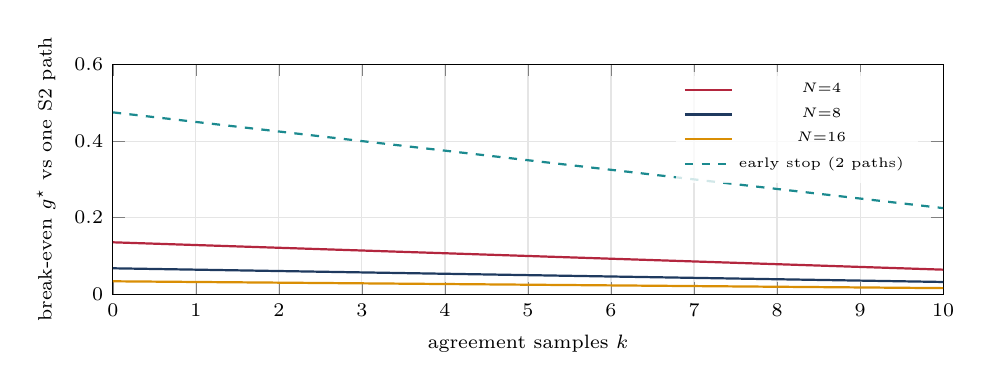
\begin{tikzpicture}
\begin{axis}[xlabel={agreement samples $k$},ylabel={break-even $g^{\star}$ vs one S2 path},xmin=0,xmax=10,ymin=0,ymax=0.6,legend pos=north east]
\addplot[crimson,thick,domain=0:10]{(1-0.05*(1+x))/(4*1.75)};\addlegendentry{$N{=}4$}
\addplot[navy,thick,domain=0:10]{(1-0.05*(1+x))/(8*1.75)};\addlegendentry{$N{=}8$}
\addplot[amber,thick,domain=0:10]{(1-0.05*(1+x))/(16*1.75)};\addlegendentry{$N{=}16$}
\addplot[teal,thick,dashed,domain=0:10]{(1-0.05*(1+x))/2};\addlegendentry{early stop (2 paths)}
\end{axis}
\end{tikzpicture}

\scriptsize\textbf{Amendment:} define the Phase-1 baseline (S2 with the same loop, or report the cost--accuracy frontier); use $n{=}4$ in one request for the $k$ samples.
\end{columns}
\end{frame}

\begin{frame}{T4 -- The router is a threshold rule}
\begin{columns}[T]
\column{.52\textwidth}
\begin{theorem}[T4]\small
Let $e_1(s)=\Pr[\text{S1 wrong}\mid s]$, $e_2(s)=\Pr[\text{final wrong after S2}\mid s]$, $L$ = error cost, $c_{esc}$ = extra escalation cost. Optimal: escalate iff
$e_1(s)-e_2(s)>c_{esc}/L$; a single threshold $\tau$ if the gap is monotone.
\end{theorem}
\small\textit{Proof.} Answer: $Le_1$. Escalate: $c_{esc}+Le_2$. Compare. $\square$

\textbf{Quantile adaptation (DKW).} Realised $g$ within $\varepsilon$ of $g^{\star}$ w.p.\ $1-\delta$ if $n\ge\ln(2/\delta)/(2\varepsilon^2)$: $n{=}512\Rightarrow\varepsilon{=}.06$; $\varepsilon{=}.02$ needs $4{,}611$.
\begin{alertblock}{Diagnostic conflict}
\scriptsize If $\tau$ tracks a target $g$, then $g$ is constant by construction and cannot show learning. Fix $\tau$ (cost formula) and watch $g$ fall, \emph{or} fix $g$ and watch S1 pass rate $m$ rise.
\end{alertblock}
\column{.48\textwidth}
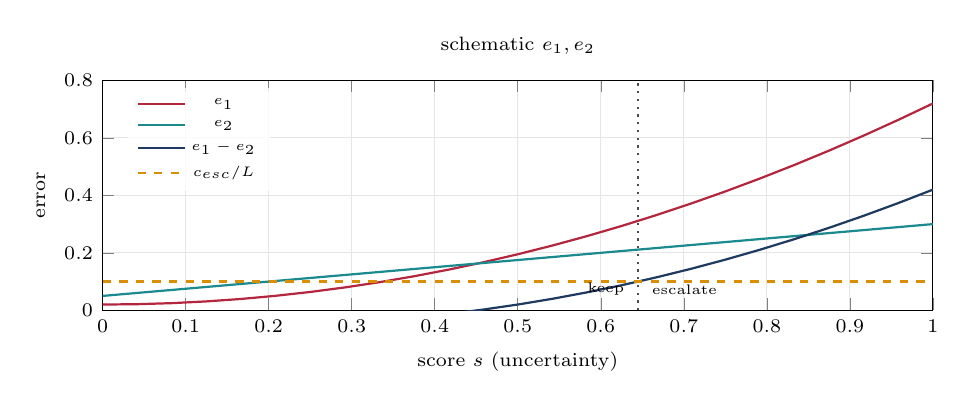
\begin{tikzpicture}
\begin{axis}[xlabel={score $s$ (uncertainty)},ylabel={error},xmin=0,xmax=1,ymin=0,ymax=0.8,legend pos=north west,title={\scriptsize schematic $e_1,e_2$}]
\addplot[crimson,thick,domain=0:1]{0.02+0.7*x^2};\addlegendentry{$e_1$}
\addplot[teal,thick,domain=0:1]{0.05+0.25*x};\addlegendentry{$e_2$}
\addplot[navy,thick,domain=0:1]{0.02+0.7*x^2-0.05-0.25*x};\addlegendentry{$e_1-e_2$}
\addplot[amber,dashed,thick]coordinates{(0,0.1)(1,0.1)};\addlegendentry{$c_{esc}/L$}
\addplot[black!70,dotted,thick]coordinates{(0.645,0)(0.645,0.8)};
\node[font=\tiny,anchor=south west] at (axis cs:0.65,0.02){escalate};
\node[font=\tiny,anchor=south east] at (axis cs:0.64,0.02){keep};
\end{axis}
\end{tikzpicture}

\scriptsize\textbf{Amendments:} one calibrated score (logistic on labelled tasks) instead of separate $H,A$; estimate $e_2$ (correlated with $e_1$, same family); \texttt{mean\_entropy} is a truncated top-5 proxy, so 0.35 nats is not meaningful until calibrated.
\end{columns}
\end{frame}

\begin{frame}{T5 -- Consensus arithmetic and its limit}
\begin{columns}[T]
\column{.55\textwidth}
\begin{theorem}[T5]\small
$\text{consensus}(c)=k/(N{-}1)$, $k$ = other candidates agreeing. $\text{consensus}\ge\theta\iff k\ge\lceil\theta(N{-}1)\rceil$.\\
$N{=}8$: $\theta{=}.75$ needs 7 of 8 agreeing; $\theta{=}.9$ needs 8 of 8. $N{=}4$: both need 4 of 4.\\
$\Pr[\text{unanimous and wrong}]\le p_{\max}^{N-1}(1-q)$ per task.
\end{theorem}
\begin{alertblock}{Limit}
\small Averaged over tasks this tends to the mass of tasks where the model \emph{deterministically} errs. It does not vanish as $N$ grows.
\end{alertblock}
\column{.45\textwidth}
\small
\textbf{Consequences}
\begin{itemize}
\item $V_{\min}{=}0.9$ applied to consensus silently means unanimity
\item Express consensus in candidate counts
\item Keep \texttt{assurance=consensus} flagged
\item Never write memory or training data from consensus without human check
\item Pseudo-code \texttt{ceil(theta*(N-1))+1} must state whether \texttt{agree\_count} includes the candidate itself
\end{itemize}
\end{columns}
\end{frame}

\begin{frame}{T6 -- Value score algebra}
\begin{columns}[T]
\column{.5\textwidth}
\begin{theorem}[T6]\small
$V=0.5\min(h,a)+0.25u+0.25m$ on $[0,1]^4$.\\
(i) $V\ge.7$ does not imply the gate: $h{=}.49$, $a{=}u{=}m{=}1$ gives $.745$.\\
(ii) Vacuous hedge $h{=}a{=}m{=}1,u{=}0$ gives $.75\ge V_{\min}$.
\end{theorem}
\small\textit{Proof.} Substitute. $\square$

\textbf{Amendment.} Explicit gate $h,a\ge.5$ and helpfulness floor $u\ge.5$, plus $V\ge.7$. Per-verifier $V_{\min}$: 1.0 for exact verifiers (code, schema), 0.9 for soft ones.
\column{.5\textwidth}
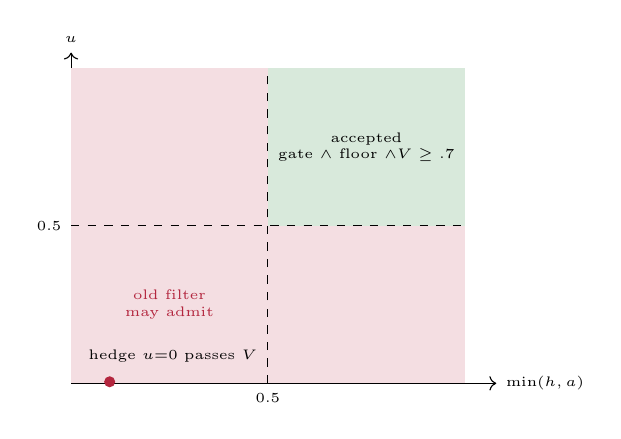
\begin{tikzpicture}[x=1cm,y=1cm]
\draw[->](0,0)--(5.4,0)node[right,font=\tiny]{$\min(h,a)$};\draw[->](0,0)--(0,4.2)node[above,font=\tiny]{$u$};
\fill[crimson!15](0,0)rectangle(2.5,4);\fill[crimson!15](0,0)rectangle(5,2);
\fill[green!20](2.5,2)rectangle(5,4);
\node[font=\tiny,align=center] at (3.75,3){accepted\\ gate $\wedge$ floor $\wedge V\ge.7$};
\node[font=\tiny,align=center,text=crimson] at (1.25,1){old filter\\ may admit};
\fill[crimson](0.5*0.98,4*0.0+0.02) circle(2pt);
\node[font=\tiny,anchor=west] at (0.1,0.35){hedge $u{=}0$ passes $V$};
\draw[dashed](2.5,0)--(2.5,4);\draw[dashed](0,2)--(5,2);
\node[font=\tiny,below] at (2.5,0){0.5};\node[font=\tiny,left] at (0,2){0.5};
\end{tikzpicture}
\end{columns}
\end{frame}

\begin{frame}{T7 -- Coupling between System 1 and System 2}
\begin{columns}[T]
\column{.55\textwidth}
\begin{theorem}[T7]\small
If \texttt{sample\_paths} does not read the S1 draft, then
$$\Pr[\text{S2 adopts wrong draft}\mid\text{draft wrong}]=\sum_{a\in\text{wrong}}P_1(a)P_2(a),$$
the collision probability of two independent answer laws. Passing the draft adds anchoring on top. Certifying adoption $<5\%$ at 95\% with zero observed needs $n\ge\ln .05/\ln .95$, i.e.\ 59 trials; with $f$ adoptions use Clopper--Pearson.
\end{theorem}
\small\textbf{Amendment:} System~2 is \emph{draft-blind} by default; draft-conditioned mode is an ablation; run the coupling test on both with $\ge200$ trials. Same model family $\Rightarrow$ collision probability is not small: measure it.
\column{.45\textwidth}
\centering
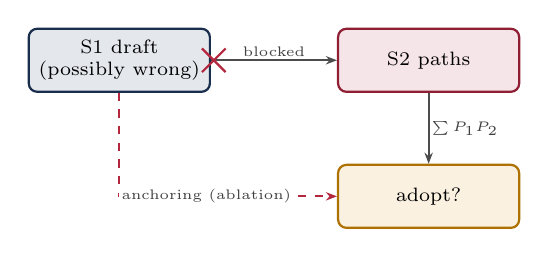
\begin{tikzpicture}[x=1cm,y=1cm]
\node[blk=navy](d){S1 draft\\ (possibly wrong)};
\node[blk=crimson,right=1.6cm of d](p){S2 paths};
\node[blk=amber,below=0.9cm of p](x){adopt?};
\draw[arr](d)--node[lab,above]{blocked}(p);
\draw[dsh,crimson](d.south)|-node[lab,pos=.7]{anchoring (ablation)}(x.west);
\draw[arr](p)--node[lab,right]{$\sum P_1P_2$}(x);
\draw[thick,crimson](1.05,0.15)--(1.35,-0.15);\draw[thick,crimson](1.05,-0.15)--(1.35,0.15);
\end{tikzpicture}
\end{columns}
\end{frame}

\begin{frame}{T8 -- Self-model bias under routing}
\begin{columns}[T]
\column{.54\textwidth}
\begin{theorem}[T8]\small
\texttt{s2\_pass} is observed only on escalated tasks, i.e.\ those where S1 failed: the naive estimate is $\Pr[\text{correct}\mid\text{S1 failed}]$. Audit a random fraction $\epsilon$ of non-escalated tasks with S2. Then
$\hat p_2=g\,\hat p_{2|esc}+(1-g)\,\hat p_{2|audit}$ is unbiased (IPW, positivity $\epsilon>0$), with
$\mathrm{SE}\le\sqrt{\tfrac{g^2p(1-p)}{ng}+\tfrac{(1-g)^2p(1-p)}{n(1-g)\epsilon}}$.
\end{theorem}
\small $n{=}10^4,g{=}.3,\epsilon{=}.05$: 350 audited, $\mathrm{SE}\le0.019$.
\vspace{2pt}

\textbf{Also:} non-verifiable domains are \emph{unmeasured}, not 0.0; key stats by adapter hash with a sliding window.
\column{.46\textwidth}
\centering
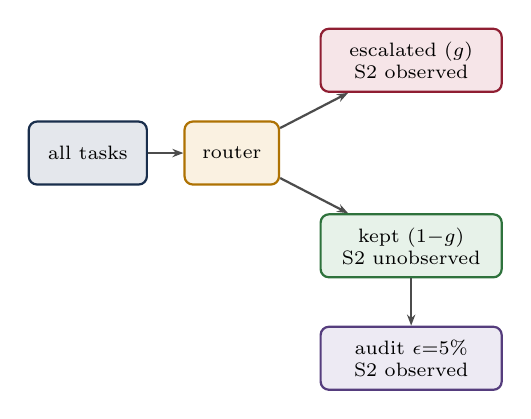
\begin{tikzpicture}[x=1cm,y=1cm]
\node[blk=navy,minimum width=1.5cm](all){all tasks};
\node[blk=amber,minimum width=1.2cm,right=0.45cm of all](r){router};
\node[blk=crimson,minimum width=2.3cm,above right=0.35cm and 0.5cm of r](e){escalated ($g$)\\ S2 observed};
\node[blk=green,minimum width=2.3cm,below right=0.35cm and 0.5cm of r](k){kept ($1{-}g$)\\ S2 unobserved};
\node[blk=violet,minimum width=2.3cm,below=0.6cm of k](au){audit $\epsilon{=}5\%$\\ S2 observed};
\draw[arr](all)--(r);\draw[arr](r)--(e);\draw[arr](r)--(k);\draw[arr](k)--(au);
\end{tikzpicture}
\end{columns}
\end{frame}

\begin{frame}{T9, T10 -- Measurement floors of the evaluation suite}
\begin{columns}[T]
\column{.62\textwidth}
\scriptsize
\begin{tabular}{@{}p{1.9cm}p{1.2cm}p{2.1cm}p{2.1cm}@{}}
\toprule
Gate & Spec & Problem & Needed\\\midrule
Escalation rate & 500 & $\pm6.1$ pts & 4,611 for $\pm2$\\
ECE $\le.08$ & 500, 10 bins & noise floor 0.034 & 5,700 (10 bins) / 2,900 (5) or debias\\
Presence $\le10\%$ & 100 & obs.\ 10\% $\Rightarrow$ UB .16 & $\ge500$\\
Flying Man $\ge.90$ & 30 & 27/30 $\Rightarrow$ LB .76 & $\ge60$\\
Coupling $\le5\%$ & not stated & 59 with 0 hits & 200\\
P1 non-inferior (1 pt) & 500 & resolves 3.5 pts & 6,200 pairs ($\delta{=}.1$); 690 for 3 pts\\
Drift & $K{=}50$, $\alpha{=}.05$ & 2.6 false alarms/yr & $K\ge(2.487\sigma/\Delta)^2$; $\alpha{=}.01$/CUSUM\\\bottomrule
\end{tabular}
\column{.38\textwidth}
\begin{block}{Formulas}
\scriptsize
ECE bias for calibrated outputs:\\
$\E[\widehat{\mathrm{ECE}}]\approx\sqrt{\tfrac2\pi}\sqrt{\bar p(1{-}\bar p)}\sqrt{B/n}$.\\[2pt]
Non-inferiority: $n\ge(z_\alpha{+}z_\beta)^2\delta/m^2$, with $z_\alpha{+}z_\beta{=}2.487$.\\[2pt]
Drift: effective sample is $K$ (probe pairs correlated); $\sigma{=}.1\Rightarrow K{\ge}25$; $\sigma{=}.2\Rightarrow K{\ge}99$.
\end{block}
\scriptsize Add a \emph{negative control} (shuffled/contradictory commitments): embedding cosine measures wording more than stance.
\end{columns}
\end{frame}

\begin{frame}{T11 -- Distillation: noise, measured gain, gate size}
\begin{columns}[T]
\column{.58\textwidth}
\begin{theorem}[T11]\small
(a) If a fraction $\eta$ of labels is wrong, $|\mathrm{err}_{noisy}(h)-\mathrm{err}_{clean}(h)|\le\eta$ for every $h$; here $\eta=\rho$ of T1.\\
(b) Eval verifier $(r,\varphi)$: measured rate $=\varphi+(r-\varphi)t$, so a measured $+2$ pts is a true $+2/(r-\varphi)$ pts; training on verifier-accepted outputs can raise $\varphi$ (Goodhart) and inflate it.\\
(c) Paired gate, discordance $\delta$: $n\ge z^2\delta/\varepsilon^2$. $\delta{=}.1,\varepsilon{=}.01$: 2,706 per domain; Bonferroni over 5 ($z{=}2.326$): 5,410.
\end{theorem}
\small\textit{Proof (a).} The events differ only where the noisy label is wrong. \hfill$\square$
\column{.42\textwidth}
\begin{alertblock}{Amended promotion gate}
\small
\begin{itemize}\setlength\itemsep{0pt}
\item lower bound of overall gain $>0$, point estimate $\ge2$ pts
\item lower bound of each domain change $\ge-1$ pt
\item eval on a verifier never used in collection
\item keep 5\% abstain examples
\item ECE, Flying Man, presence still pass
\item human sign-off; hash into self-model
\end{itemize}
\end{alertblock}
\end{columns}
\end{frame}

\begin{frame}{T12 -- Serving capacity}
\begin{columns}[T]
\column{.5\textwidth}
\begin{theorem}[T12]\small
KV bytes per sequence $=2\,L_{kv}H_{kv}d_{head}\,b\,T$, where $L_{kv}$ counts layers that keep a KV cache. S2 tokens in flight $=N(\text{prompt}+\text{generated})$.
\end{theorem}
\small\textbf{Illustration} (hypothetical dims; read \texttt{config.json}): 64 layers, 8 KV heads, $d{=}128$, 2 B $\Rightarrow$ 0.25\,MB/token. GPU0 leaves $0.9{\cdot}80-54=18$\,GB $\approx72$K tokens; 8 paths $\times$ 16K $=131$K tokens, so paths queue or are preempted.

\textbf{Amendment.} Derive concurrency from the real config (a hybrid-attention model shrinks $L_{kv}$), then budget $N$ and \texttt{max\_tokens}, or lower $N$.
\column{.5\textwidth}
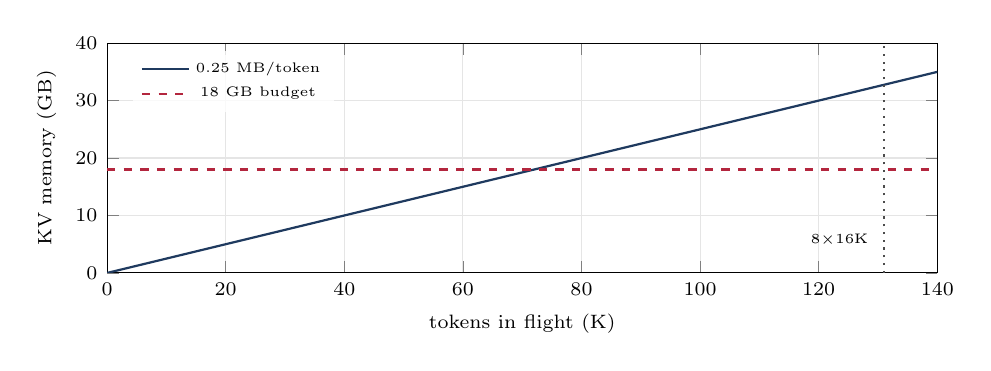
\begin{tikzpicture}
\begin{axis}[xlabel={tokens in flight (K)},ylabel={KV memory (GB)},xmin=0,xmax=140,ymin=0,ymax=40,legend pos=north west]
\addplot[navy,thick,domain=0:140]{x*0.25};\addlegendentry{0.25 MB/token}
\addplot[crimson,dashed,thick]coordinates{(0,18)(140,18)};\addlegendentry{18 GB budget}
\addplot[black!70,dotted,thick]coordinates{(131,0)(131,40)};
\node[font=\tiny,anchor=south east] at (axis cs:130,3){8$\times$16K};
\end{axis}
\end{tikzpicture}
\end{columns}
\end{frame}

\begin{frame}{P1 -- End-to-end identity (added): when is the cascade safe?}
\begin{proposition}[Cascade difference identity]\small
Let $\rho_1$ = P(wrong $\mid$ router keeps the S1 answer), and $\bar e_2^{\,kept}$ = error S2-only would make on those same tasks. If S2 behaves identically on escalated tasks in both systems, then
$$\Pr[\text{cascade wrong}]-\Pr[\text{S2-only wrong}]=(1-g)\,\bigl(\rho_1-\bar e_2^{\,kept}\bigr).$$
\end{proposition}
\vspace{-2pt}
\small\textit{Proof.} The two systems coincide on the escalated fraction $g$ and differ only on the kept fraction $1-g$. \hfill$\square$

\begin{columns}[T]
\column{.5\textwidth}
\begin{block}{Corollaries}
\scriptsize
\begin{itemize}\setlength\itemsep{1pt}
\item Non-inferiority within margin $m$ requires $\rho_1\le\bar e_2^{\,kept}+m/(1-g)$; e.g.\ $m{=}.01,g{=}.3$: $\rho_1\le\bar e_2^{\,kept}+1.4$ pts.
\item $\bar e_2^{\,kept}$ is observable only through audits (T8): the audit stream is part of the safety case, not telemetry.
\item With a verifier on kept answers, $\rho_1$ is T1's $\rho$: control $\varphi$.
\end{itemize}
\end{block}
\column{.5\textwidth}
\centering
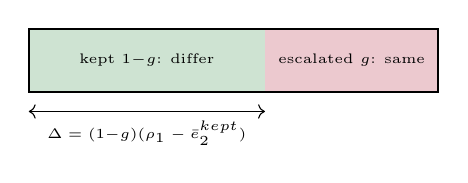
\begin{tikzpicture}[x=1cm,y=1cm]
\fill[green!25](0,0)rectangle(3.0,0.8);\fill[crimson!25](3.0,0)rectangle(5.2,0.8);
\draw[thick](0,0)rectangle(5.2,0.8);
\node[font=\tiny] at (1.5,0.4){kept $1{-}g$: differ};\node[font=\tiny] at (4.1,0.4){escalated $g$: same};
\draw[<->](0,-0.25)--node[below,font=\tiny]{$\Delta=(1{-}g)(\rho_1-\bar e_2^{kept})$}(3.0,-0.25);
\end{tikzpicture}
\end{columns}
\end{frame}

\section{Part III: Technical report}

\begin{frame}{Defect register and amendments}
\scriptsize
\begin{tabular}{@{}c p{4.6cm} c p{6.2cm}@{}}
\toprule
\# & Defect & Result & Amendment\\\midrule
1 & Cascade not cheaper vs same-loop S2 unless $g$ small & T3 & define baseline; early stop; $n{=}4$ agreement call\\
2 & 500-task baseline too small & T4,T9,T11 & $\ge$4,600; 6,200 for 1-pt non-inferiority\\
3 & Hard gate not coded; hedge passes & T6 & gate + helpfulness floor $u\ge.5$\\
4 & $V_{\min}{=}.9$ lets code fail 10\%; consensus = unanimity & T5 & 1.0 for exact verifiers; consensus in candidates\\
5 & $\tau$ adaptation vs $g$ diagnostic & T4 & fix cost threshold or fix $g$, not both\\
6 & Capability table biased by routing & T8 & audit $\epsilon{=}.05$; mark unmeasured\\
7 & ECE 0.08 unmeasurable at 500 & T9 & 5 bins, $n\ge2{,}900$, or debiased ECE\\
8 & S1 draft anchors S2 & T7 & draft-blind default; coupling $\ge200$\\
9 & LLM rederivation in math verifier & -- & deterministic checks only\\
10 & Router code $\ne$ prose & T4 & one calibrated score; state rule for failed verifiable\\\bottomrule
\end{tabular}
\end{frame}

\begin{frame}{Amended decision flow}
\centering
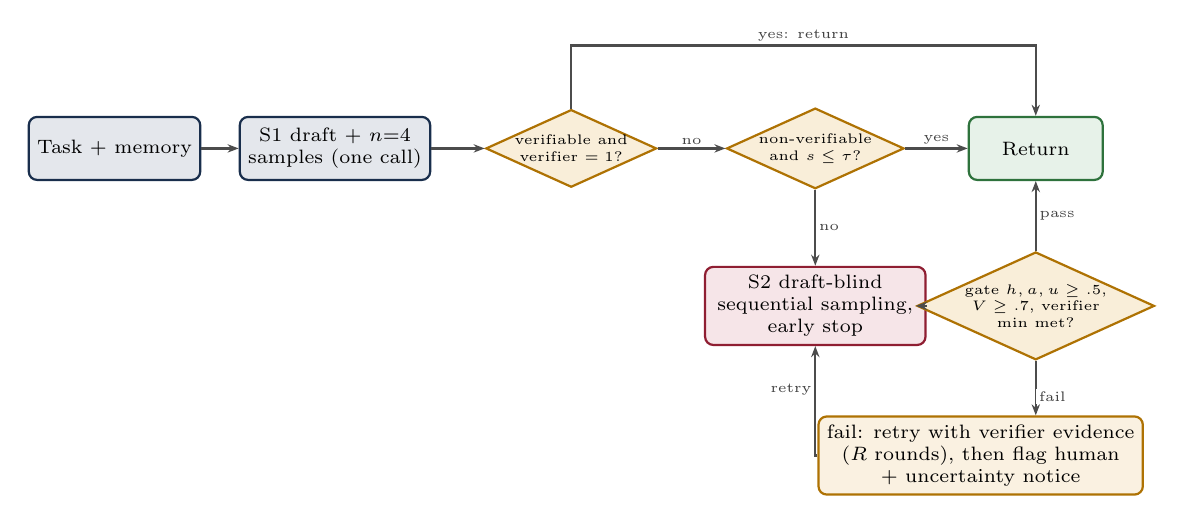
\begin{tikzpicture}[x=1cm,y=1cm,
dm/.style={diamond,aspect=2.2,draw=amber!80!black,fill=amber!15,thick,font=\tiny,align=center,inner sep=0pt}]
\node[blk=navy,minimum width=1.9cm](t) at (0,0){Task + memory};
\node[blk=navy,minimum width=2.4cm](s1) at (2.8,0){S1 draft + $n{=}4$\\ samples (one call)};
\node[dm](v) at (5.8,0){verifiable and\\ verifier $=1$?};
\node[dm](c) at (8.9,0){non-verifiable\\ and $s\le\tau$?};
\node[blk=green,minimum width=1.7cm](ret) at (11.7,0){Return};
\node[blk=crimson,minimum width=2.8cm](s2) at (8.9,-2.0){S2 draft-blind\\ sequential sampling,\\ early stop};
\node[dm](g) at (11.7,-2.0){gate $h,a,u\ge.5$,\\ $V\ge.7$, verifier\\ min met?};
\node[blk=amber,minimum width=3.4cm](fl) at (11.0,-3.9){fail: retry with verifier evidence\\ ($R$ rounds), then flag human\\ + uncertainty notice};
\draw[arr](t)--(s1);\draw[arr](s1)--(v);
\draw[arr](v)--node[lab,above]{no}(c);
\draw[arr](c)--node[lab,above]{yes}(ret);
\draw[arr](v.north)--++(0,0.8)-|node[lab,pos=.25,above]{yes: return}(ret.north);
\draw[arr](c)--node[lab,right]{no}(s2);
\draw[arr](s2)--(g);
\draw[arr](g)--node[lab,right]{pass}(ret);
\draw[arr](g.south)--(g.south |- fl.north);
\node[lab,right] at (11.7,-3.15){fail};
\draw[arr](fl.west)-|node[lab,pos=.8,left]{retry}(s2.south);
\end{tikzpicture}

\vspace{2pt}\scriptsize A verifiable task that fails verification is not eligible for the entropy shortcut and escalates (resolves defect 10). Every return is logged; 5\% of kept tasks also get an S2 audit (T8).
\end{frame}

\begin{frame}[fragile]{Amended selection code (replaces the \texttt{ok} filter)}
\begin{lstlisting}
def accept(c, task):
    if c.honesty < 0.5 or c.harm_avoidance < 0.5 or c.helpfulness < 0.5:
        return False                       # hard gate + helpfulness floor
    if c.value_score < VAL_MIN:            # 0.7
        return False
    if task.verifiable:
        return c.verifier_score >= c.verifier_min   # 1.0 for exact verifiers
    # non-verifiable: count in candidates, flag assurance=consensus
    return c.agree_count >= math.ceil(THETA * (N - 1))
\end{lstlisting}
\begin{columns}[T]
\column{.5\textwidth}\scriptsize
\textbf{Selection among accepted}: sort by calibrated score only if it adds information beyond the pass bit (T2); otherwise uniform.
\column{.5\textwidth}\scriptsize
\textbf{Math verifier}: SymPy or numeric equality against a reference. No LLM rederivation, preserving ``verifiers are not LLMs''.
\end{columns}
\end{frame}

\begin{frame}{Features and capabilities}
\begin{columns}[T]
\column{.5\textwidth}
\begin{exampleblock}{Features}
\small
\begin{itemize}\setlength\itemsep{1pt}
\item Dual-process routing with calibrated score
\item Verified best-of-$N$ with early stop and evidence-fed retries
\item Verifier hub: code sandbox, SymPy, JSON Schema, citation check; each with $(r,\varphi)$
\item Rubric value core with hard gate and drift monitor
\item Memory: episodic, semantic (verified only), procedural; provenance in prompt
\item Metrics-only self-model; nightly presence check
\item Gated weekly LoRA distillation of verified traces
\end{itemize}
\end{exampleblock}
\column{.5\textwidth}
\begin{block}{Capabilities (what it can deliver)}
\small
\begin{itemize}\setlength\itemsep{1pt}
\item Verified answers on code, math, schema tasks, with precision bounded by T1
\item Calibrated abstention and flagged uncertainty elsewhere
\item Stable, measurable self-description
\item Gradually cheaper operation as S1 absorbs verified skill
\end{itemize}
\end{block}
\begin{alertblock}{Honest limits}
\small
Non-verifiable domains stay at consensus assurance (T5); S1/S2/judge errors are correlated (shared family); no consciousness claim.
\end{alertblock}
\end{columns}
\end{frame}

\begin{frame}{Revised constants}
\centering\small
\begin{tabular}{@{}lll@{}}
\toprule
Parameter & Current & Proposed\\\midrule
Phase 0 baseline & 500 tasks & $\ge$4,600; 6,200 for 1-pt non-inferiority (700 for 3 pts)\\
ECE & 10 bins, $n{=}500$ & 5 bins with $n\ge2{,}900$, or debiased\\
Presence questions & 100 & $\ge500$\\
Flying Man probes & 30 & $\ge60$\\
Coupling trials & not stated & $\ge200$, draft-blind and conditioned\\
Code / schema $V_{\min}$ & 0.9 & 1.0 (soft verifiers 0.9)\\
Helpfulness floor & none & 0.5\\
Audit rate $\epsilon$ & none & 0.05\\
Drift test & $\alpha=.05$ & $\alpha=.01$ or CUSUM + negative control\\
Promotion gate & point estimates & confidence bounds, held-out verifier\\\bottomrule
\end{tabular}

\vspace{4pt}\scriptsize All values remain functions of Phase 0 measurements, not fixed targets.
\end{frame}

\begin{frame}[fragile]{Self-model and value drift loop}
\begin{columns}[T]
\column{.5\textwidth}
\begin{lstlisting}
capabilities:   # updater.py only
  code: {s1_pass: .., s2_pass: ..,
         ece: .., n: .., adapter: <hash>}
  math: {...}
  factual: unmeasured   # not 0.0
limits:        # from measured failures
goals:         # human-edited only
commitments:   # human-edited only
\end{lstlisting}
\scriptsize Sliding window keyed by adapter hash; S2 gets $\le$2,000 tokens, S1 a 200-token digest.
\column{.5\textwidth}
\centering
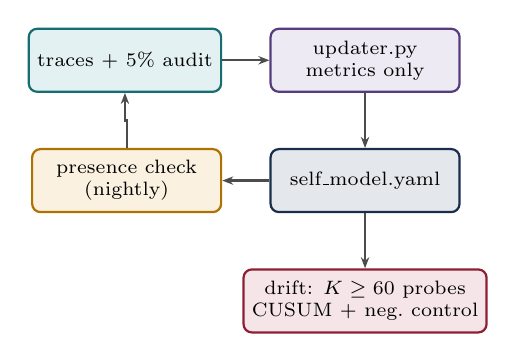
\begin{tikzpicture}[x=1cm,y=1cm]
\node[blk=teal,minimum width=2.4cm](tr){traces + 5\% audit};
\node[blk=violet,minimum width=2.4cm,right=0.6cm of tr](up){updater.py\\ metrics only};
\node[blk=navy,minimum width=2.4cm,below=0.7cm of up](sm){self\_model.yaml};
\node[blk=amber,minimum width=2.4cm,left=0.6cm of sm](pc){presence check\\ (nightly)};
\node[blk=crimson,minimum width=2.4cm,below=0.7cm of sm](dr){drift: $K\ge60$ probes\\ CUSUM + neg.\ control};
\draw[arr](tr)--(up);\draw[arr](up)--(sm);\draw[arr](sm)--(pc);\draw[arr](pc.north)--++(0,0.35)-|(tr.south);
\draw[arr](sm)--(dr);
\end{tikzpicture}
\end{columns}
\end{frame}

\begin{frame}{Distillation loop (substantial motion)}
\centering
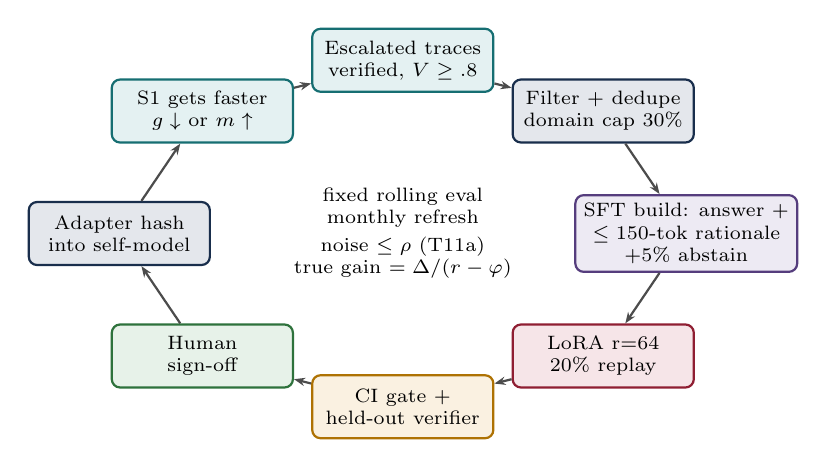
\begin{tikzpicture}[x=1cm,y=1cm]
\foreach \idx/\txt/\col/\ang in {
 1/{Escalated traces\\ verified, $V\ge.8$}/teal/90,
 2/{Filter + dedupe\\ domain cap 30\%}/navy/45,
 3/{SFT build: answer +\\ $\le150$-tok rationale\\ +5\% abstain}/violet/0,
 4/{LoRA r=64\\ 20\% replay}/crimson/-45,
 5/{CI gate +\\ held-out verifier}/amber/-90,
 6/{Human\\ sign-off}/green/-135,
 7/{Adapter hash\\ into self-model}/navy/180,
 8/{S1 gets faster\\ $g\downarrow$ or $m\uparrow$}/teal/135}
 {\node[blk=\col,minimum width=2.3cm](n\idx) at (\ang:3.6cm and 2.2cm){\txt};}
\foreach \i/\j in {1/2,2/3,3/4,4/5,5/6,6/7,7/8,8/1}{\draw[arr](n\i)--(n\j);}
\node[font=\scriptsize,align=center] at (0,0){fixed rolling eval\\ monthly refresh\\[2pt] noise $\le\rho$ (T11a)\\ true gain $=\Delta/(r-\varphi)$};
\end{tikzpicture}
\end{frame}

\begin{frame}{Development plan (re-baselined)}
\centering
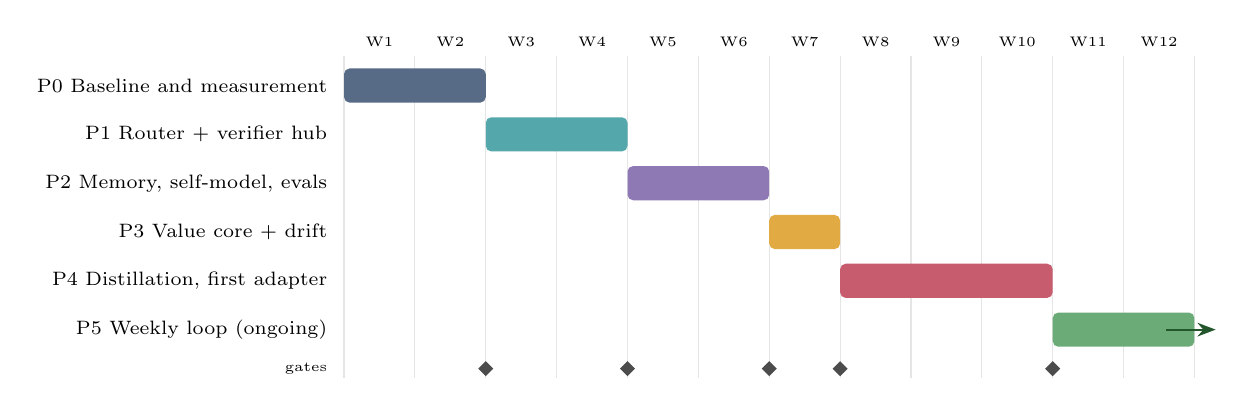
\begin{tikzpicture}[x=0.9cm,y=0.62cm]
\foreach \w in {1,...,12}{\node[font=\tiny] at (\w-0.5,0.7){W\w};\draw[black!10](\w-1,0.4)--(\w-1,-6.2);}
\draw[black!10](12,0.4)--(12,-6.2);
\foreach \ii/\lbl/\st/\en/\col in {
 0/{P0 Baseline and measurement}/0/2/navy,
 1/{P1 Router + verifier hub}/2/4/teal,
 2/{P2 Memory, self-model, evals}/4/6/violet,
 3/{P3 Value core + drift}/6/7/amber,
 4/{P4 Distillation, first adapter}/7/10/crimson,
 5/{P5 Weekly loop (ongoing)}/10/12/green}
 {\node[anchor=east,font=\scriptsize] at (-0.1,-\ii-0.2){\lbl};
  \fill[\col!75,rounded corners=2pt](\st,-\ii-0.55) rectangle (\en,-\ii+0.15);}
\draw[-{Stealth},thick,green!60!black](11.6,-5.2)--(12.3,-5.2);
\foreach \x in {2,4,6,7,10}{\node[diamond,fill=black!70,inner sep=1.4pt] at (\x,-6.0){};}
\node[anchor=east,font=\tiny] at (-0.1,-6.0){gates};
\end{tikzpicture}

\scriptsize Phase 0 grows from 1 to 2 weeks to reach the $\ge$4,600-task floor; later phases shift by one week (proposed). Each diamond is a gate on the next slide.
\end{frame}

\begin{frame}{Phase gates (amended)}
\scriptsize\centering
\begin{tabular}{@{}p{2.3cm}p{5.0cm}p{6.0cm}@{}}
\toprule
Phase & Deliverable & Acceptance\\\midrule
P0 & Serve both models; $\ge$4,600-task multi-domain run of S1-only and S2-only & Stable endpoints; estimates of $q$, $(r,\varphi)$, $e_1(s),e_2(s)$, $c_1/c_p$, $\delta$, KV capacity\\
P1 & Router, verifier hub (code, math, schema) with mutation tests & Cost below S2 \emph{with same loop}, accuracy loss within 1 pt at 95\% (6,200 pairs) or 3 pts (700)\\
P2 & Memory, self-model updater, audit stream, Flying Man, presence & Both tests end to end; $\ge60$ probes, $\ge500$ questions; coupling $\ge200$ trials\\
P3 & Value core, drift monitor & Baseline $P_S$, measured $\sigma$, negative control separates, alerts fire\\
P4 & Distillation pipeline, first adapter & Confidence-bound gate passes; human sign-off\\
P5 & Weekly collect, train, gate, promote & Gate each cycle; weekly 2\% human audit of judge\\\bottomrule
\end{tabular}
\end{frame}

\begin{frame}{Risk register}
\scriptsize\centering
\begin{tabular}{@{}p{3.2cm}p{4.3cm}p{5.6cm}@{}}
\toprule
Risk & Mechanism & Mitigation\\\midrule
Version drift & Qwen releases fast; embed/rerank unverified & Pin revisions and templates; re-baseline on any change\\
Correlated errors & S1, S2, judge share family (A1, A2 fail) & Independent verifiers; human audit; measure collision (T7)\\
Verifier false accepts & $\rho$ set by $\varphi$ (T1) & Mutation testing; per-verifier $V_{\min}$; private test set\\
Goodhart in distillation & $\varphi$ rises when training on accepted outputs & Held-out verifier; confidence-bound gate (T11)\\
Self-model bias & Selection by routing (T8) & 5\% audit; unmeasured flag; adapter-keyed window\\
KV exhaustion & $N\times$16K tokens exceed budget (T12) & Config-derived concurrency; lower $N$ or tokens\\
Non-verifiable assurance & consensus has a floor (T5) & Flag; prefer abstain; human check before reuse\\
MoE LoRA tooling & expert-layer support uncertain & Attention-only LoRA fallback; dense S1 fallback\\\bottomrule
\end{tabular}
\end{frame}

\begin{frame}{Conclusion and open items}
\begin{columns}[T]
\column{.5\textwidth}
\begin{block}{Conclusion}
\small
Nafs-Aql is a coherent, buildable design on Qwen. Its soundness rests on three quantities that must be measured, not assumed: verifier false-accept $\varphi$, router calibration $e_1(s),e_2(s)$, and S1/S2 error correlation. With the ten amendments, every gate is both implementable and statistically resolvable.
\end{block}
\column{.5\textwidth}
\begin{alertblock}{Open items (Phase 0 outputs)}
\small
\begin{itemize}\setlength\itemsep{1pt}
\item $q$ per domain; $(r,\varphi)$ per verifier
\item $e_1,e_2$; $c_1/c_p$; discordance $\delta$; drift $\sigma$
\item real KV capacity from \texttt{config.json}
\item confirm 35B-A3B card, embedding/reranker versions, any newer Qwen release
\end{itemize}
\end{alertblock}
\end{columns}
\end{frame}

\end{document}
